
%----------------------------------------------------------------------------------------
%	PACKAGES AND DOCUMENT CONFIGURATIONS
%----------------------------------------------------------------------------------------

\documentclass{article}

\usepackage{fullpage}
%\usepackage{mhchem} % Package for chemical equation typesetting
%\usepackage{siunitx} % Provides the \SI{}{} command for typesetting SI units

\usepackage{graphicx} % Required for the inclusion of images

\setlength\parindent{0pt} % Removes all indentation from paragraphs

\renewcommand{\labelenumi}{\alph{enumi}.} % Make numbering in the enumerate environment by letter rather than number (e.g. section 6)

%\usepackage{times} % Uncomment to use the Times New Roman font

%----------------------------------------------------------------------------------------
%	DOCUMENT INFORMATION
%----------------------------------------------------------------------------------------

\title{Monte Carlo Studies on the Effect of Detector Casings on Incident Energy Spectra} % Title

\author{Tom Stainer} % Author name

\date{\today} % Date for the report

\begin{document}

\maketitle % Insert the title, author and date

%----------------------------------------------------------------------------------------
%	ABSTRACT
%----------------------------------------------------------------------------------------
\begin{abstract}A GEANT4 simulation is used to describe a basic setup in which a casing plate of customised aluminium composition is instrumented with a flat energy spectrum of incident neutron and gammas in the energy range of 0.2 - 15 MeV. Different thicknesses of the aluminium casing are implemented, ranging from 6 to 30 mm in thickness. Isotropic sources of neutrons and gammas are used with rates and energies recorded upon leaving the casing. In the energy region of 0.2 to 2 MeV neutron efficiencies $\geq$ 94\% and gamma efficiencies exceeding 80\% can be achieved for one layer of the aluminium casing design. In the higher energy range, $>$2 MeV, particle efficiencies exceed 98\%. Efficiencies for Carbon Fiber and Lead casings of 1, 3 and 5 mm are also presented for comparison.
\end{abstract}

\newpage
%----------------------------------------------------------------------------------------
%	SECTION 1 - INTRO
%----------------------------------------------------------------------------------------

\section{Introduction}
Special Nuclear Materials (Highly Enriched Uranium and Plutonium) are difficult to detect. Detection and identification becomes even more difficult when shielding or detector casing is instrumented. Such barriers introduce extra unwanted material which alter the energies of the particles emitted from the source. An accurate description of how such instrumentation effects the incident spectra on the detectors is required to aid identification of nuclear material. Simulations are a key tool in providing a solution to this problem by modelling how neutrons and gammas propagate and interact with matter.


%----------------------------------------------------------------------------------------
%	SECTION 2 - SETUP and procedure
%----------------------------------------------------------------------------------------

\section{Setup and Procedure}

For the detector design in MODES-SNM weight is a key factor, the requirement in the project restricts the total weight of each detector unit to 25 kg. It is then necessary to have a very light but supportive structure and casing for the detectors. Aluminium is a perfect candidate for this due to its low density and relative strength. It is also an excellent electrical conductor helping eliminate electric noise. In order to provide the correct level of support while keeping to the weight restrictions, the design of the casing consists of a honeycomb aluminium structure sandwiched between two thin aluminium sheets.
\newline
\begin{figure}[htbp]
\begin{center}
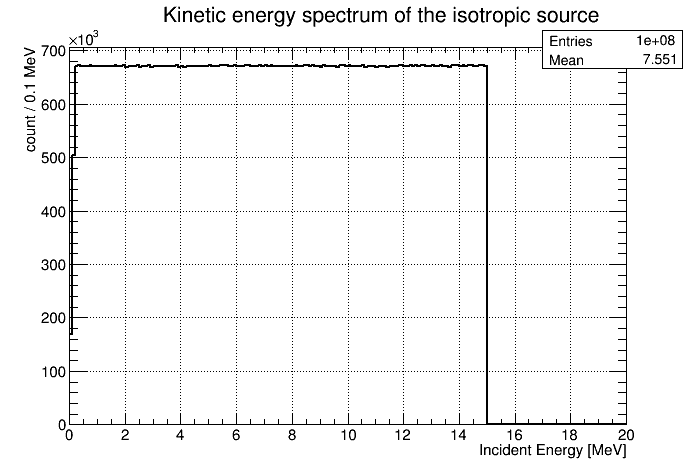
\includegraphics[width=100mm]{figures/kineticEnergySpectrum.png}
\caption{Kinetic energy spectrum of the neutrons and gammas incident on the casing.}
\label{fig:incidentEnergy}
\end{center}
\end{figure}

\begin{figure}[htbp]
\begin{center}
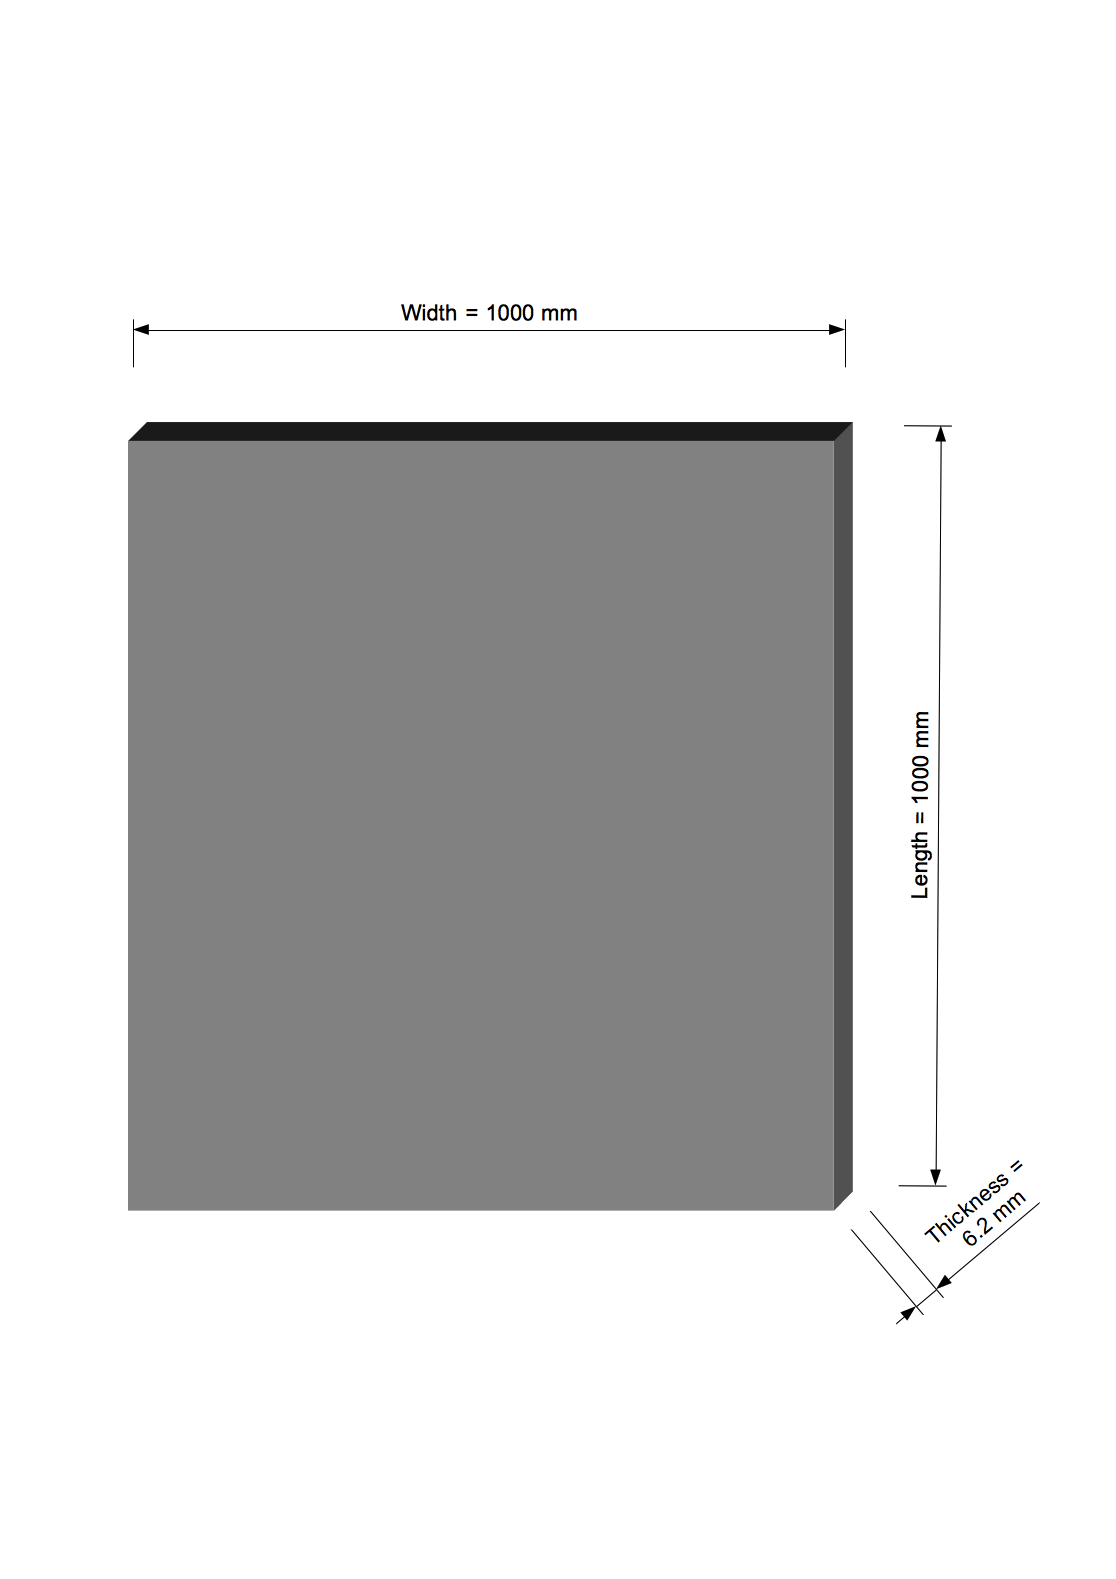
\includegraphics[width=70mm]{figures/casingDiagram1.png}
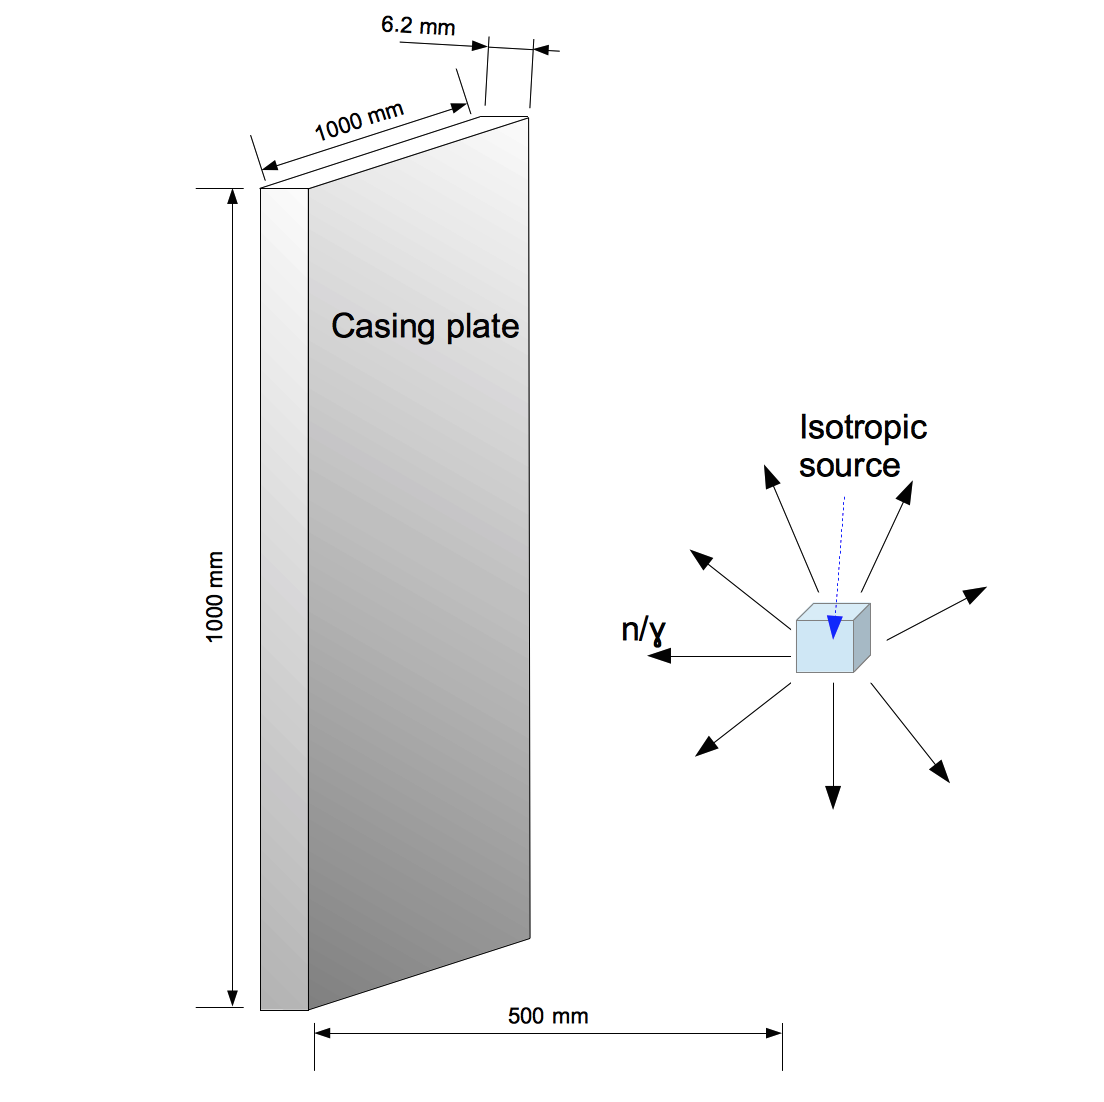
\includegraphics[width=70mm]{figures/setupDiagram1.png}
\caption{One layer of the casing plate of aluminium with dimension labels (left) and the experimental setup (right).}
\label{fig:casingDiagram}
\end{center}
\end{figure}

Monte Carlo simulations are implemented to gain an understanding of the effects such a casing would introduce to the incident energy spectra of neutrons and gammas. Geant4\cite{geant4} is used to study particle interactions within the casing and record information on these for large amounts of events. A hypothetical source with a flat and isotropic energy spectrum ranging from 0.2 to 15 MeV is implemented in the simulation to best study the energy range of interest for the MODES-SNM project, figure~\ref{fig:incidentEnergy}. The source is implemented at a distance of 0.5 m from the casing with source dimensions of 1 $\times$ 1 $\times$ 1 $cm^{3}$. One layer of the casing is modelled as a solid sheet of 1.0 mm thick aluminium (100\% $^{27}_{13}$Al), density 2.7 $gcm^{-3}$, on top of a sheet of the same aluminium composition but with 5.2 mm thickness and a lower density of 0.29 $gcm^{-3}$. Resulting in a thickness of 6.2 mm for one layer, while the length and width of the casing plate have dimensions of 1 m $\times$ 1 m, shown on the left of figure~\ref{fig:casingDiagram}. The source and casing plate are situated in a vacuum with the complete experimental setup shown on the right of figure~\ref{fig:casingDiagram}. 
\newline

Only information on the primary particle is of interest for this study and tracking is setup to propagate the primary until it is either outside the main experimental boundaries or it is absorbed. The particles kinetic energy, momentum and position are recorded upon reaching the casing and once more upon leaving the casing. With this information and using particle and event identification, it is possible to calculate the energy deposition in the casing from the difference of kinetic energies of the particle leaving the casing from entering the casing. All primaries are recorded that pass through the casing boundary, defined in the simulation as a step into that volume, wether energy is deposited or not. 1 $\times$ 10$^{8}$ primary particles are generated at the source, with around a sixth of this, $\sim$1.6 $\times$ 10$^{7}$, reaching the casing boundary. 

%----------------------------------------------------------------------------------------
%	SECTION 3- Particle Interactions
%----------------------------------------------------------------------------------------

\section{Particle Interactions}
The energy deposition in the casing as a function of incident energy is shown in figure~\ref{fig:energyDep}, for both neutrons and gammas for 1, 2 and 3 layers of the aluminium. It is noticeable in the neutron plots that a structure can be seen in 1 layer but slowly fades out with the introduction of more material. This is due to kinematic restrictions from elastic scattering of the neutron off Aluminium, which neutrons can only transfer up to 14\% of their kinetic energy per scatter. This is easier to notice when taking the energy ratios of kinetic energy of neutrons leaving the casing and the initial kinetic energy of the neutrons incident on the casing, left in figure~\ref{fig:energyRatio}. The kinetic energies of the primaries entering and leaving the casing are shown separately in figure~\ref{fig:inOutFlux} also.

\begin{figure}[htbp]
\begin{center}
\includegraphics[width=80mm]{figures/220813/neutron1Layer_energy2D.png}
\includegraphics[width=80mm]{figures/220813/gamma1Layer_energy2D.png}
\includegraphics[width=80mm]{figures/220813/neutron2Layer_energy2D.png}
\includegraphics[width=80mm]{figures/220813/gamma2Layer_energy2D.png}
\includegraphics[width=80mm]{figures/220813/neutron3Layer_energy2D.png}
\includegraphics[width=80mm]{figures/220813/gamma3Layer_energy2D.png}
\caption{The neutron (left) and gamma (right) energy deposition as a function of incident energy for 1 (top), 2 (middle) and 3 layers (bottom).}
\label{fig:energyDep}
\end{center}
\end{figure}


\begin{figure}[htbp]
\begin{center}
\includegraphics[width=80mm]{figures/220813/neutronEnergyRatio.png}
\includegraphics[width=80mm]{figures/220813/gammaEnergyRatio.png}
\caption{The ratio of kinetic energies for the neutrons (left) and gammas (right) upon leaving the casing to entering it for 1,2,3,4 and 5 layers of the casing.}
\label{fig:energyRatio}
\end{center}
\end{figure}

\begin{figure}[htbp]
\begin{center}
\includegraphics[width=80mm]{figures/220813/neutronAl1LayerInOutEnergies.png}
\includegraphics[width=80mm]{figures/220813/gammaAl1LayerInOutEnergies.png}
\caption{The neutron and gamma energy spectra upon entering and leaving the aluminium casing of 1 layer.}
\label{fig:inOutFlux}
\end{center}
\end{figure}

\newpage
%----------------------------------------------------------------------------------------
%	SECTION 4- Efficiencies
%----------------------------------------------------------------------------------------

\section{Casing Efficiencies}
In order to quantify the effect of the casing, efficiencies as a function of kinetic energy are calculated by equation~\ref{eq:efficiency}.

\begin{equation}
\textnormal{efficiency, } \epsilon = \frac{\textnormal{histogram of original kinetic energies of the particles leaving the casing boundary}} {\textnormal{histogram of original kinetic energies of the particles incident on casing boundary}}
\label{eq:efficiency}
\end{equation}

\subsection{Examining different numbers of layers}
In the current detector housing design some of the detectors are positioned such that 5 layers of the casing would be located in front of them. It is then necessary to measure the effect that this would have on the energy spectra. To give a comparison of introducing additional layers numbers of 1,2,3,4 and 5 layers are shown in figures~\ref{fig:efficienciesAlLayers} and \ref{fig:efficienciesAlLayersZoom}.

\begin{figure}[htbp]
\begin{center}
\includegraphics[width=80mm]{figures/220813/neutronAlEfficiencyAllLayers0o2MeVBinning.png}
\includegraphics[width=80mm]{figures/220813/gammaAlEfficiencyAllLayers0o2MeVBinning.png}
\caption{The neutron and gamma efficiencies for 1,2,3,4 and 5 layers of the aluminium casing.}
\label{fig:efficienciesAlLayers}
\end{center}
\end{figure}

\begin{figure}[htbp]
\begin{center}
\includegraphics[width=80mm]{figures/220813/neutronAlEfficiencyAllLayersZoom.png}
\includegraphics[width=80mm]{figures/220813/gammaAlEfficiencyAllLayersZoom.png}
\caption{The neutron and gamma efficiencies for 1,2,3,4 and 5 layers of the aluminium casing in the energy region of 0 - 2 MeV.}
\label{fig:efficienciesAlLayersZoom}
\end{center}
\end{figure}

\subsection{Other Materials}
Other potential candidates for casing materials are also considered in the detector casing design. The two other materials tested are Carbon Fiber ($C_{3}H_{3}N$) and Lead (100\% $^{207}_{82}$Pb). These are tested for casings of 1,3 and 5 mm thicknesses with their associated efficiencies shown in figure~\ref{fig:efficienciesMaterial}. 

\begin{figure}[htbp]
\begin{center}
\includegraphics[width=75mm]{figures/230713/neutronAll1mmMaterialEfficiency.png}
\includegraphics[width=75mm]{figures/230713/gammaAll1mmMaterialEfficiency.png}
\includegraphics[width=75mm]{figures/230713/neutronAll3mmMaterialEfficiency.png}
\includegraphics[width=75mm]{figures/230713/gammaAll3mmMaterialEfficiency.png}
\includegraphics[width=75mm]{figures/230713/neutronAll5mmMaterialEfficiency.png}
\includegraphics[width=75mm]{figures/230713/gammaAll5mmMaterialEfficiency.png}
\caption{The neutron (left) and gamma (right) efficiencies for casings of 1 (top), 3 (middle) and 5 mm (bottom) thicknesses of Carbon Fiber and Lead.}
\label{fig:efficienciesMaterial}
\end{center}
\end{figure}

\begin{figure}[htbp]
\begin{center}
\includegraphics[width=75mm]{figures/230713/neutronAll1mmMaterialEfficiencyZoom.png}
\includegraphics[width=75mm]{figures/230713/gammaAll1mmMaterialEfficiencyZoom.png}
\includegraphics[width=75mm]{figures/230713/neutronAll3mmMaterialEfficiencyZoom.png}
\includegraphics[width=75mm]{figures/230713/gammaAll3mmMaterialEfficiencyZoom.png}
\includegraphics[width=75mm]{figures/230713/neutronAll5mmMaterialEfficiencyZoom.png}
\includegraphics[width=75mm]{figures/230713/gammaAll5mmMaterialEfficiencyZoom.png}
\caption{The neutron (left) and gamma (right) efficiencies for casings of 1 (top), 3 (middle) and 5 mm (bottom) thicknesses of Carbon Fiber and Lead for lower energies between 0 and 2 MeV.}
\label{fig:efficienciesMaterialZoom}
\end{center}
\end{figure}
\newpage
%----------------------------------------------------------------------------------------
%	SECTION 5- Conclusions
%----------------------------------------------------------------------------------------

\section{Conclusions}
In MODES neutrons of around 1 MeV are of key interest and it can be seen that efficiencies of 97\% can be achieved for 1 layer of the aluminium casing. This falls to 91\% for the same energy but for 3 layers of the material. Comparing this with other materials it shows this Aluminium casing can provide higher efficiencies than Carbon fiber and Lead for both neutrons and gammas. In the higher energy range ($\sim$ 8 MeV and above for neutrons) Carbon Fiber is more efficient but however it is an extremely expensive material to produce and such benefits do not provide good reason to increase the project costs. 
%----------------------------------------------------------------------------------------
%	BIBLIOGRAPHY
%----------------------------------------------------------------------------------------

\bibliographystyle{unsrt}

%\bibliography{sample}
\begin{thebibliography}{9}
\bibitem{geant4}
  S. Agostinelli et al,
  \emph{Geant4: a simulation toolkit}.
  NIM A, vol. 506, no. 3, pp. 250-303, 2003

\end{thebibliography}
%----------------------------------------------------------------------------------------


\end{document}